\ifdefined\ishandout
\documentclass[handout]{beamer}
\else
\documentclass{beamer}
\fi

%\usepackage[frenchb]{babel}
\usepackage[T1]{fontenc}
%\usepackage[utf8]{inputenc}
\usepackage{hyperref}
\usepackage{multirow}
\usepackage{listings}
\usepackage{fancyvrb}
\usepackage{tikz}
\usepackage{framed}
\usepackage{xmpmulti}

\usepackage{algorithm}
\usepackage{algorithmicx}
\usepackage{algpseudocode}
\usepackage{xcolor}
\usepackage{booktabs}
\usepackage{color, colortbl}
\ifdefined\ishandout
\usepackage{handoutWithNotes}
\fi
\usepackage{slashbox}
\usepackage{amsmath}
\usepackage{bm}
\usepackage{hhline}
\usepackage{pgfplots}
\usepackage{caption}

\def\UrlBreaks{\do\/\do-}

\usetikzlibrary{shapes.geometric}
\usetikzlibrary{positioning}
\usetikzlibrary{shapes.arrows, chains}
\usetikzlibrary{arrows,calc}
\usetikzlibrary{shapes.multipart}
\usetikzlibrary{matrix}

\usepackage{array}
%\usetheme{Boadilla}
\usetheme[progressbar=frametitle]{metropolis}

\usefonttheme[onlymath]{serif}

\newcommand{\R}{\mathbb{R}}
%\newcommand{\C}{\mathbb{C}}
\newcommand{\N}{\mathbb{N}}
\newcommand{\Z}{\mathbb{Z}}
\newcommand{\E}{\mathbb{E}}
\newcommand{\Var}{\text{Var}}
\newcommand{\Cov}{\text{Cov}}
\ifdefined\ishandout
\pgfpagesuselayout{3 on 1 with notes}[a4paper,border shrink=5mm]
\usecolortheme{dove}
\else
%\usecolortheme{dolphin}
%\usecolortheme{crane}
\fi

\metroset{block=fill}

\lstnewenvironment{codeC}
{ \lstset{language=C,
    otherkeywords={printf,scanf}}
}
{}

\ifdefined\ishandout
\definecolor{mygreen}{rgb}{0,0,0}
\definecolor{mymauve}{rgb}{0,0,0}
\definecolor{myblue}{rgb}{0,0,0}
\else
\definecolor{mygreen}{rgb}{0,0.6,0}
\definecolor{mymauve}{rgb}{0.58,0,0.82}
\definecolor{myblue}{rgb}{0,0,1}

\fi

%% Notes
%\setbeameroption{show only notes}


\definecolor{mygray}{rgb}{0.5,0.5,0.5}

\lstset{ language=Python,%
  backgroundcolor=\color{white},   % choose the background color; you must add \usepackage{color} or \usepackage{xcolor}
  basicstyle=\footnotesize,        % the size of the fonts that are used for the code
  breakatwhitespace=false,         % sets if automatic breaks should only happen at whitespace
  breaklines=true,                 % sets automatic line breaking
  captionpos=b,                    % sets the caption-position to bottom
  commentstyle=\color{mygreen},    % comment style
  deletekeywords={...},            % if you want to delete keywords from the given language
  escapeinside={\%*}{*)},          % if you want to add LaTeX within your code
  extendedchars=true,              % lets you use non-ASCII characters; for 8-bits encodings only, does not work with UTF-8
  frame=tb,	                   % adds a frame around the code
  keepspaces=true,                 % keeps spaces in text, useful for keeping indentation of code (possibly needs columns=flexible)
  keywordstyle=\color{blue},       % keyword style
  otherkeywords={*,...},           % if you want to add more keywords to the set
  numbers=none,                    % where to put the line-numbers; possible values are (none, left, right)
  numbersep=5pt,                   % how far the line-numbers are from the code
  numberstyle=\tiny\color{mygray}, % the style that is used for the line-numbers
  rulecolor=\color{black},         % if not set, the frame-color may be changed on line-breaks within not-black text (e.g. comments (green here))
  showspaces=false,                % show spaces everywhere adding particular underscores; it overrides 'showstringspaces'
  showstringspaces=false,          % underline spaces within strings only
  showtabs=false,                  % show tabs within strings adding particular underscores
  stepnumber=2,                    % the step between two line-numbers. If it's 1, each line will be numbered
  stringstyle=\color{mymauve},     % string literal style
  tabsize=3,	                   % sets default tabsize to 2 spaces
  title=\lstname                   % show the filename of files included with \lstinputlisting; also try caption instead of title
}
%\lstset{language=Python,
% breakatwhitespace=false,         % sets if automatic breaks should only happen at whitespace
%  breaklines=true,                 % sets automatic line breaking
%  captionpos=b,                
%%commentstyle=\itshape\color{mymauve},
%%keywordstyle=\bfseries\color{myblue},
%numbers=left,                    % where to put the line-numbers; possible values are (none, left, right)
%  numbersep=8pt,                   % how far the line-numbers are from the code
%  numberstyle=\tiny\color{mygray}, % the style that is used for the line-numbers
%%  rulecolor=\color{black},         % if not set, the frame-color may be changed on line-breaks within not-black text (e.g. comments (green here))
%  showspaces=false,                % show spaces everywhere adding particular underscores; it overrides 'showstringspaces'
%%  showstringspaces=false,          % underline spaces within strings only
%  showtabs=false,                  % show tabs within strings adding particular underscores
%  stepnumber=2,                    % the step between two line-numbers. If it's 1, each line will be numbered
%%  stringstyle=\color{mygreen},     % string literal style
%  tabsize=2 
%}
\ifdefined\ishandout
\newcommand{\red}{\textbf}
\else
\newcommand{\red}{\textcolor{red}}
\fi
%\newcommand \emph
%Default size : 12.8 cm * 9.6 cm

\newcommand{\tmark}[1]{\tikz[remember picture, baseline=-.5ex]{\coordinate(#1);}}

\definecolor{bluegreen}{RGB}{0,149,182}


%\newcommand{\output}[1]{
\setbeamertemplate{navigation symbols}{}
\newcommand{\bvrb}{\Verb[commandchars=£µ§,formatcom=\color{bluegreen}]}
\newcommand{\footvrb}{\footnotesize\Verb}
\newcommand{\vrbalert}[2][]{\visible<#1>{#2}}
%%% Commande pour les listes/arbres
\newcommand{\mvide}{\nodepart{one} \nodepart{two}}
\newcommand{\tvide}{\nodepart{one} \nodepart{two} \nodepart{three}}
\newcommand{\rref}[1][]{\hfill{\scriptsize\textit{#1}}}

%%Fin des commandes pour les listes/arbres.



%%% Paramètres du cours (à régler)
%Numéro du cours
\newcommand{\nb}{1}

\title[Machine Learning]{Part 5: Convolutional neural networks and regularization}
\author[A. Korosov]{anton.korosov@nersc.no}
\institute[NERSC]{NERSC\\
slides+notebook:\url{https://github.com/nansencenter/nersc_ml_course}}
\date{November 2021}


\begin{document}
%%%%%%%%%%%%%%%%%%%%% SLIDES DE TITRE
\begin{frame}
\titlepage
%\centering{
%\url{http://australe.upmc.fr} (onglet EPU-C5-IGE Info Gen)}
\end{frame}

\begin{frame}{Table of contents}
  \setbeamertemplate{section in toc}[sections numbered]
  \tableofcontents[hideallsubsections]
\end{frame}

\section{What is convolutional layer?}

\begin{frame}{Convolution filter: scheme}
    "The convolution operation, simply put, is combination of element-wise product of two matrices."
    \begin{figure}
   \centering
    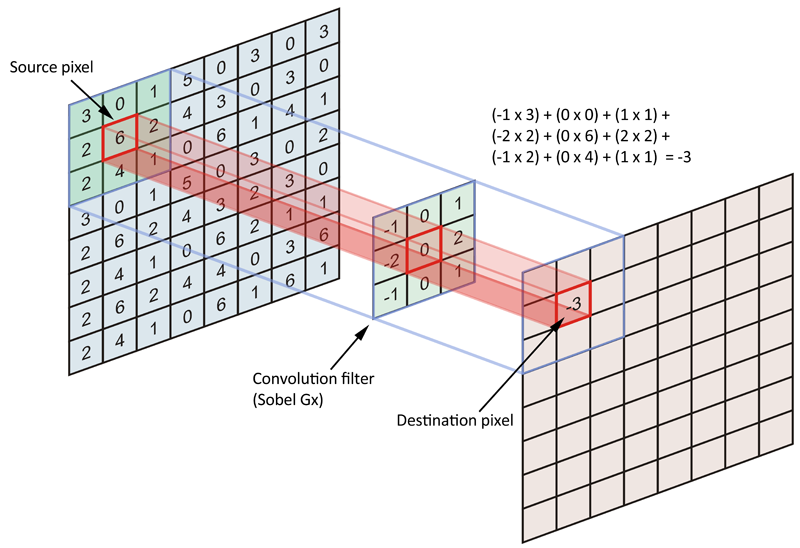
\includegraphics[width=.8\textwidth]{fig/L2/YDusp.png}
\end{figure}
{\tiny \href{https://datascience.stackexchange.com/a/23186}{ Images from Dynamic Stardust}}
\end{frame}

\begin{frame}[fragile]{Convolution filter: formula}
    \begin{tikzpicture}
    \draw[step=0.8,color=gray] (0,0) grid (4.8,4.8);
    \matrix[matrix of nodes,
    inner sep=0pt,
    anchor=south west,
    nodes={inner sep=0pt,text width=.8cm,align=center,minimum height=0.8cm}
    ]{
    $x_{11}$ & $x_{12}$ & $x_{13}$& $x_{14}$ & $x_{15}$  & $x_{16}$ \\
     $x_{21}$ & $x_{22}$ & $x_{23}$& $x_{24}$ & $x_{25}$ &  $x_{26}$ \\
    $x_{31}$ &$x_{32}$ & $x_{33}$& $x_{34}$ & $x_{35}$  & $x_{36}$ \\
    $x_{41}$ &$x_{42}$ & $x_{43}$& $x_{44}$ & $x_{45}$ & $x_{46}$  \\
     $x_{51}$ &$x_{52}$ & $x_{53}$& $x_{54}$ & $x_{55}$&  $x_{56}$  \\
     $x_{61}$ &$x_{62}$ & $x_{63}$& $x_{64}$ & $x_{65}$&  $x_{66}$  \\
    };
    \node (in) at (4.8,2.4) {} ;
    \node (out) at (8,2.4) {} ;
    \draw[step=0.8,color=gray] (8,0.8) grid (11.2,4);
    \matrix[matrix of nodes,
    xshift=8cm,
    yshift=0.8cm,
    inner sep=0pt,
    anchor=south west,
    nodes={inner sep=0pt,text width=.8cm,align=center,minimum height=0.8cm}
    ]{
    $h_{11}$ & $h_{12}$ & $h_{13}$& $h_{14}$ \\
     $h_{21}$ & $h_{22}$ & $h_{23}$& $h_{24}$ \\
    $h_{31}$ &$h_{32}$ & $h_{33}$& $h_{34}$   \\
    $h_{41}$ &$h_{42}$ & $h_{43}$& $h_{44}$  \\
    };
    
    \draw[step=0.5,color=gray] (5.999,3.499) grid (7.5,5);
    \matrix[matrix of nodes,
    xshift=5.999cm,
    yshift=3.499cm,
    inner sep=0pt,
    anchor=south west,
    nodes={inner sep=0pt,fill=orange!20,font=\footnotesize,text width=.5cm,align=center,minimum height=0.5cm}
    ]{
    $w_{11}$ & $w_{12}$ & $w_{13}$ \\
    $w_{21}$ & $w_{22}$ & $w_{23}$ \\
    $w_{31}$ & $w_{32}$ & $w_{33}$ \\
    };
    
    \path [draw, very thick, ->] (in) edge[bend left=40] 
    node [above,midway]{$\mathbf{w}$}(out);
    \node (xlabel) at (2.4,5) {$X$: an image};
    \node (hlabel) at (9.6,4.2) {$h$: first feature};
    \end{tikzpicture}
    \begin{block}{Perform a standard convolution}
    $$
    h_{i,j} = \sum_{k=1}^3\sum_{l=1}^3 x_{i+k-1,j+l-1}.w_{k,l}
    $$
    \end{block}
\end{frame}


\begin{frame}{Convolution filter of 3D input}
    Convolution of input 2D matrix with several bands is a sum of convolutions of each band $\equiv$ convolution of 3D matrix with 3D filter but only in 2 dimensions: \\
    \begin{tiny}
        Input image: $7 \times 7 \times 3$ \\
        Filter: $3 \times 3 \times 3$ \\
        Output image: $5 \times 5 \times 1$ \\
    \end{tiny}
    \begin{figure}
   \centering
    \includegraphics[width=.7\textwidth]{fig/L2/conv_filter_3d.png}
\end{figure}
{\tiny \href{https://towardsdatascience.com/a-comprehensive-guide-to-convolutional-neural-networks-the-eli5-way-3bd2b1164a53}{ Images from Sumit Saha}}
\end{frame}


\begin{frame}[t]{Main parameters of a convolutional layer}
\begin{itemize}
    \item <1-> \alert<1> {Size of the filter} $K$ 
    \item <2-> \alert<2> {Number of filters} $p$

\only<2>{
A convolutional layer is composed of $p$ convolutions (size of layer) extracting $p$ features from the data.
\begin{figure}
\centering
    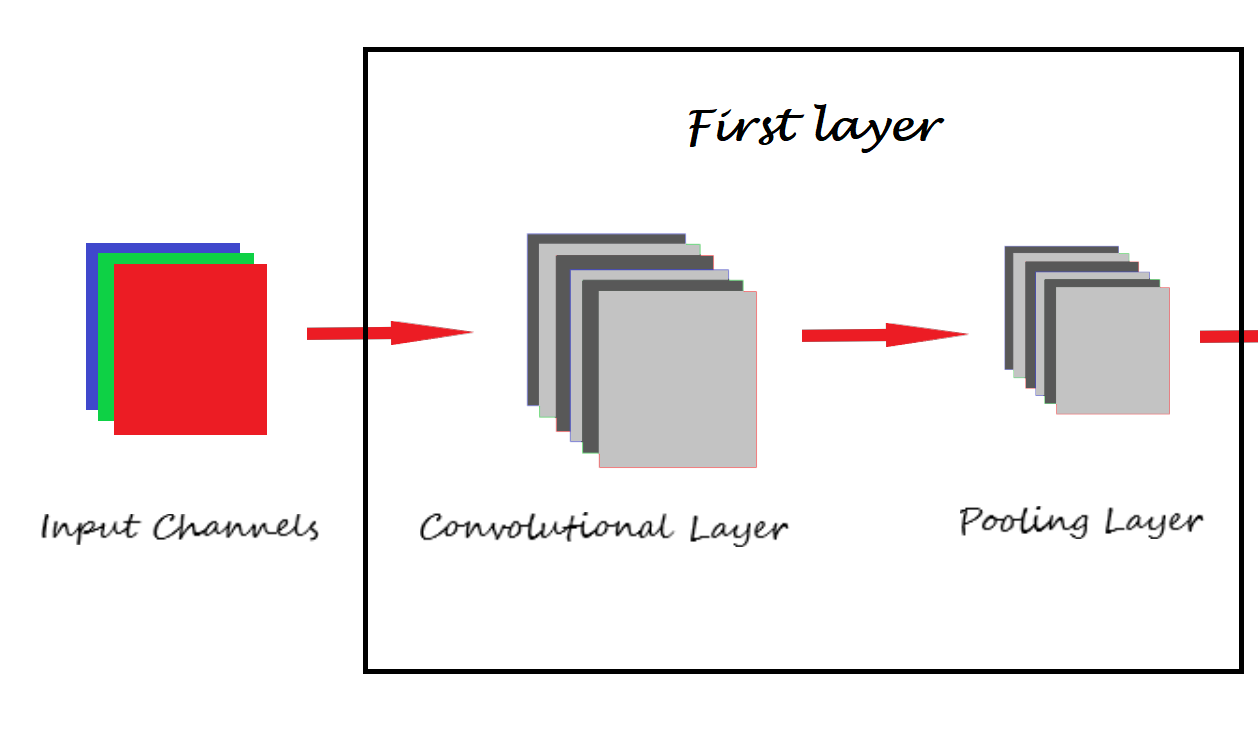
\includegraphics[width=.6\textwidth,trim={0 3.5cm 12.5cm 5cm},clip]{fig/L2/Cnn-layer.png}
\end{figure}
}

    \item <3-> \alert<3> {Strides} $S$
    
    \only<3> {
{\centering
\begin{tabular}{cc}
    $S=1$ & $S=2$ \\
    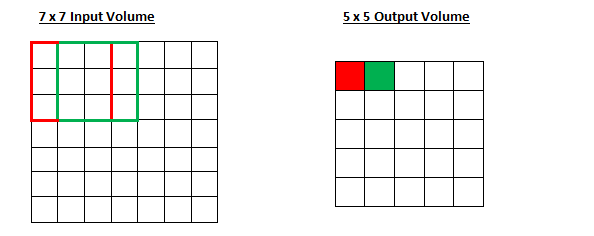
\includegraphics[trim={0.5cm 0 2.5cm 0}, clip, width=.5\textwidth]{fig/L2/Stride1.png}&
    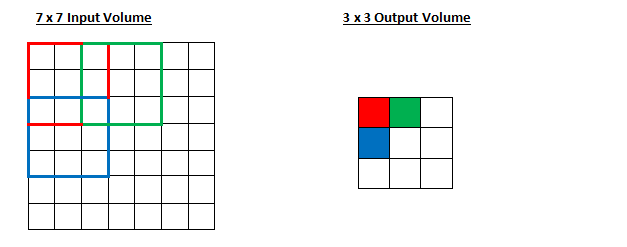
\includegraphics[trim={0 0 2.5cm 0}, clip, width=.5\textwidth]{fig/L2/Stride2.png}\\
    \end{tabular}
    }}
    
    \item <4-> \alert<4> {Padding} $P$
    
    {\only<4>
    {\centering
\begin{tabular}{cc}
    $P=1$ & $P=2$ \\
    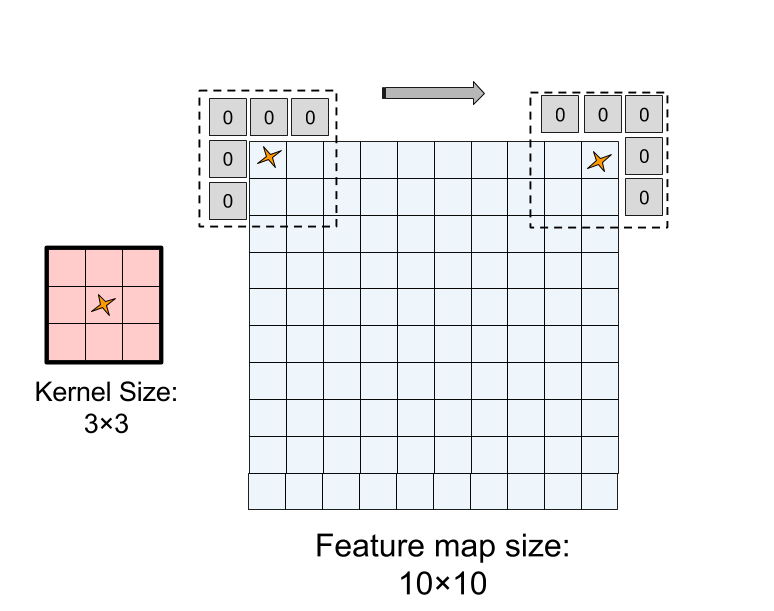
\includegraphics[trim={0 0 1.5cm 0}, clip, width=.45\textwidth]{fig/L2/pad3.png}&
    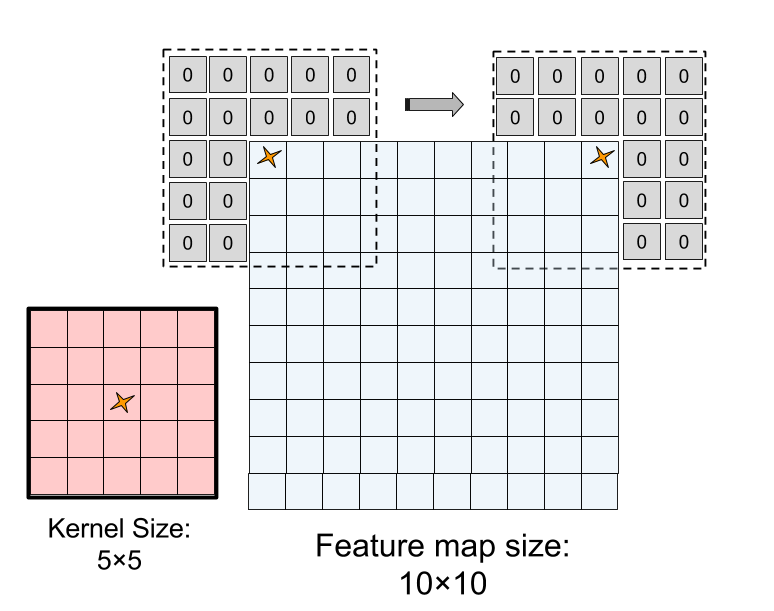
\includegraphics[trim={0 0 1.5cm 0}, clip, width=.45\textwidth]{fig/L2/pad5.png}\\
    \end{tabular}
    }

}
    
\end{itemize}
    \pause
    {\footnotesize
    $O = \frac{W - K +2P}{S} + 1$, where $O$ is the output size and $W$ the input size.
    }
\end{frame}


\begin{frame}{Summary of Convolutional layer steps}
    \begin{figure}
        \centering
        1. Convolution
\multiinclude[<+->][format=png,graphics={width=\textwidth}]{fig/L2/animated/conv}       
    \end{figure}
    \pause
    \vspace{-2em}
    \begin{columns}[t]
    \column{.7\textwidth}
    \begin{figure}
        \centering
        2. Addition
            \multiinclude[<+->][format=png,graphics={width=\textwidth}]{fig/L2/animated/channels}       

    \end{figure}
    
       \column{.3\textwidth}
       \pause
    \begin{figure}
        \centering
        3. Bias\\
\multiinclude[<+->][format=png,graphics={width=.6\textwidth}]{fig/L2/animated/bias}       
    \end{figure}
    \end{columns}
\end{frame}

\begin{frame}{Remarks on Convolutional layers}
\begin{itemize}
    \item Convolutional layers are acting locally on the image (But you can still use large scale information by adding more layers)
    \item Convolutions are invariant by translation (the weights do not depend on the location on the image).
    \item They can handle images of different sizes.
    
\end{itemize}
\end{frame}

\begin{frame}{Convolution layer notation}
    The operation of convolution, the number of filters and their size, stride and padding, and the output shape is often shown on schemes as just one "Convolution layer":  
    \begin{figure}
   \centering
    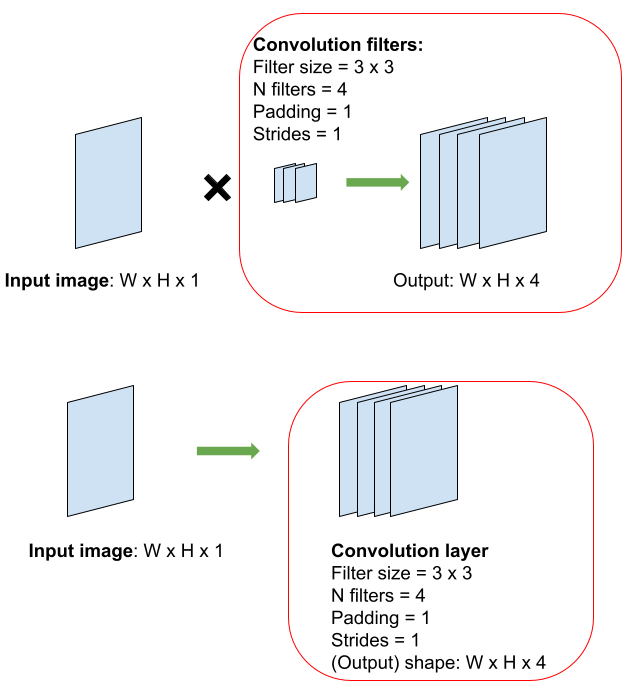
\includegraphics[width=.5\textwidth]{fig/L2/Convolutional_layer_structure_conventions.png}
\end{figure}
\end{frame}

\section{Convolutional neural networks}

\begin{frame}{Combining several convolution layers}
    Several convolution layers can be stacked to created a "deep" network. The shape of input can be preserved or reduced.
    \begin{figure}
   \centering
    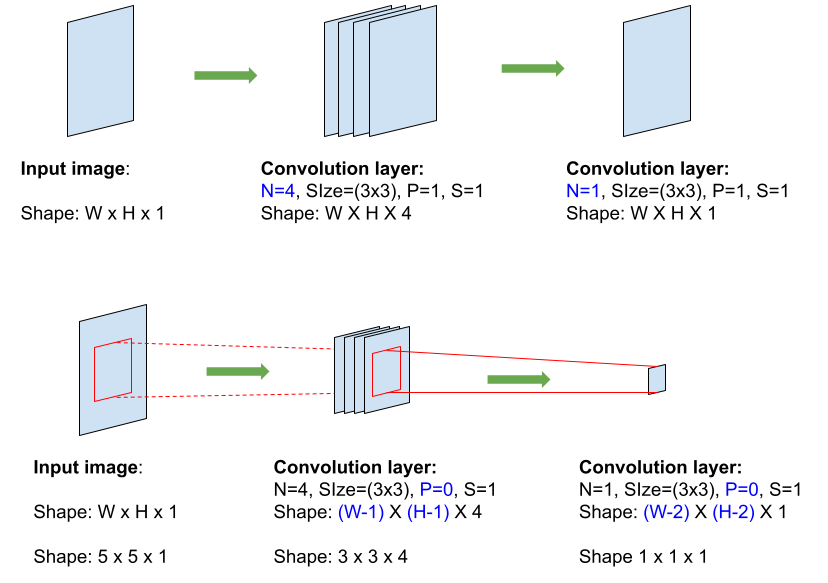
\includegraphics[width=.7\textwidth]{fig/L2/only_convolutional_layers_options.png}
\end{figure}
\end{frame}

\begin{frame}{Max-Pooling}
    In order to reduce the size of the feature space (to enhance the gradients), but to keep information from the entire input image a common operation to perform is "max-pooling".
    \begin{figure}
   \centering
    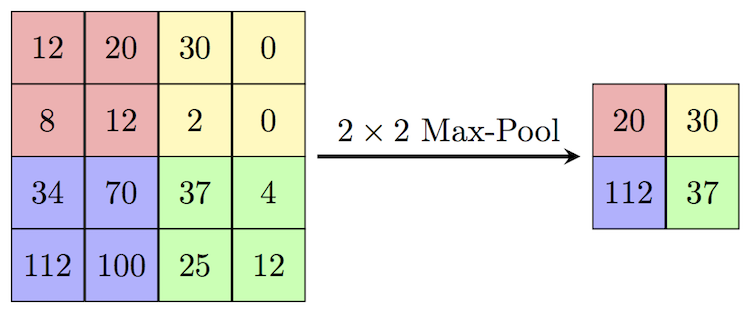
\includegraphics[width=.6\textwidth]{fig/L2/MaxpoolSample2.png}
\end{figure}
\end{frame}

\begin{frame}[fragile]{A traditional CNN architecture}
    \begin{figure}
    \centering
    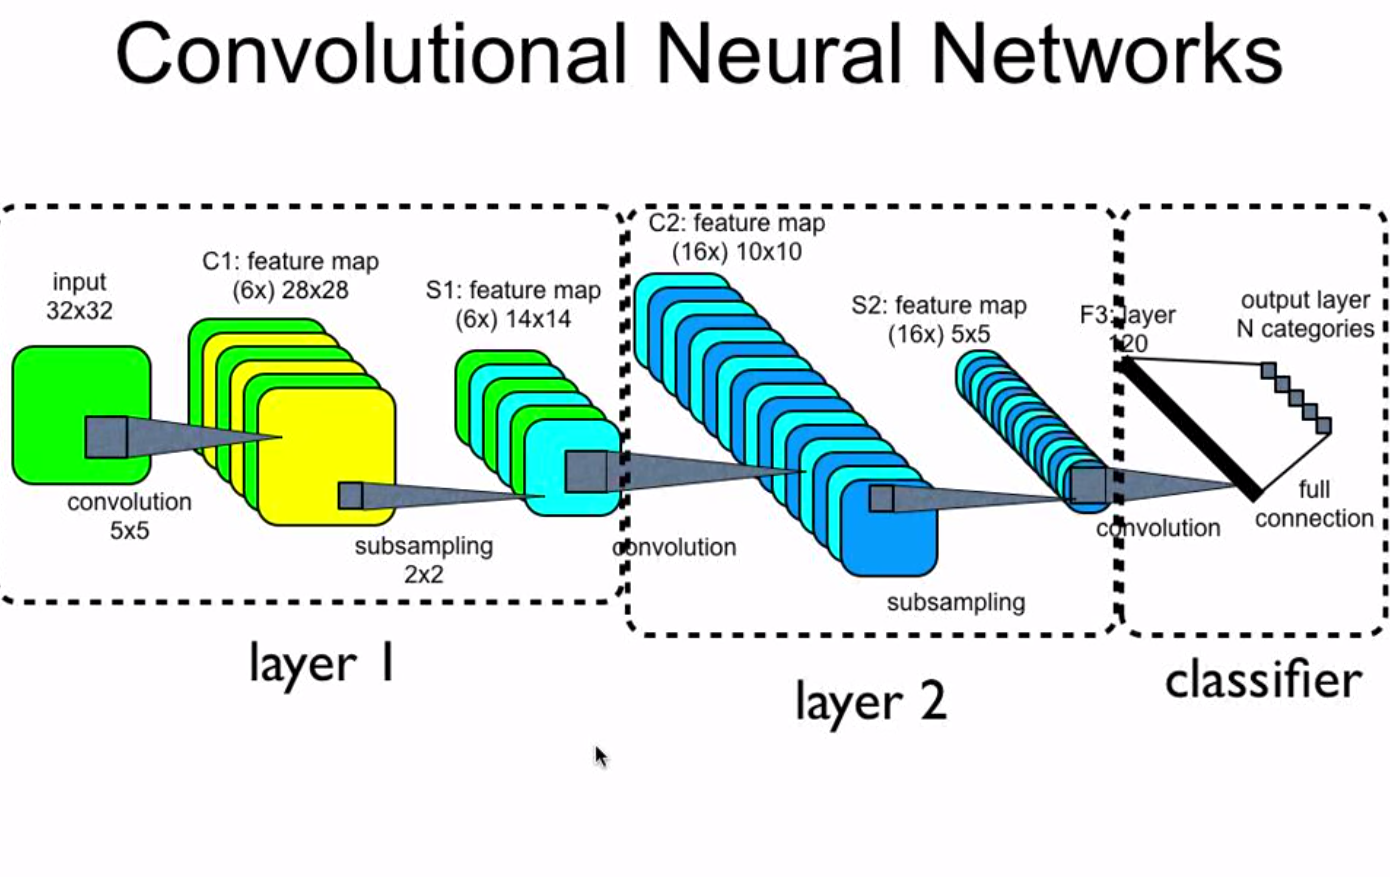
\includegraphics[width=.8\textwidth,trim={0 0cm 0cm 3cm},clip]{fig/L2/CNN.png}
    \end{figure}
Such network can be used for "image classification" tasks (is it a dog or a cat on the input image?) or "image regression" tasks (how much is the fish on the image?)
\end{frame}

\begin{frame}{Example of AlexNet}
    \alert{AlexNet} is the first Deep architecture used on ImageNet challenge in 2012 and achieved an \alert{error of 15.3\%} (10\% better than the previous best classifier). The paper was cited more than 34,000 times.

\begin{thebibliography}{GBC16}

\bibitem[KH12]{Krizhevsky2012ImageNetNetworks}
Alex Krizhevsky and Geoffrey~E Hinton, \emph{{ImageNet Classification with Deep
  Convolutional Neural Networks}}, Neural Information Processing Systems
  (2012), 1--9.

\end{thebibliography}
    \begin{figure}
        \centering
        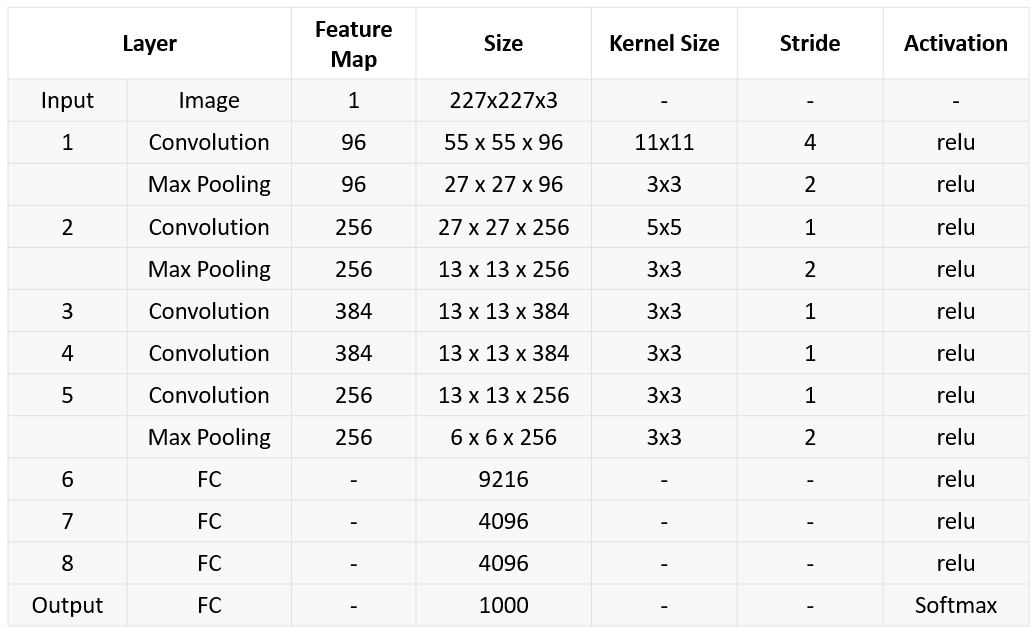
\includegraphics[width=.5\textwidth]{fig/L2/AlexNet_Summary_Table.jpg}

    \end{figure}
\end{frame}

\section{Image segmentation}

\begin{frame}{What is image segmentation?}
    When a 2D output with labels should be produced the task is called "image segmentation":
    \begin{figure}
   \centering
    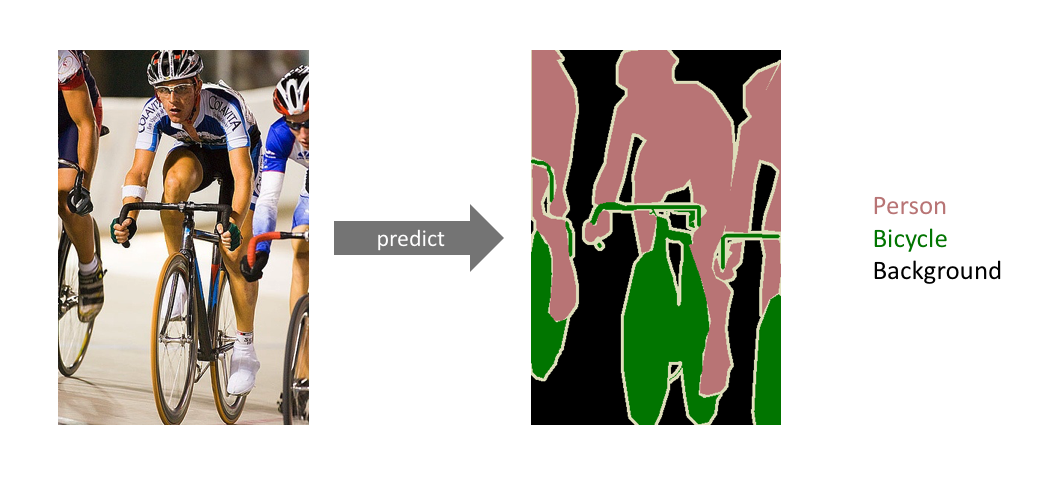
\includegraphics[width=.8\textwidth]{fig/L2/Screen-Shot-2018-05-17-at-7.42.16-PM.png}
\end{figure}
{\tiny \href{https://www.jeremyjordan.me/semantic-segmentation/}{ Images from JEREMY JORDAN}}
\end{frame}

\begin{frame}{Semantic labels}
    On a segmented image each pixel (or each patch with several pixels) is labeled with a number.
    \begin{figure}
   \centering
    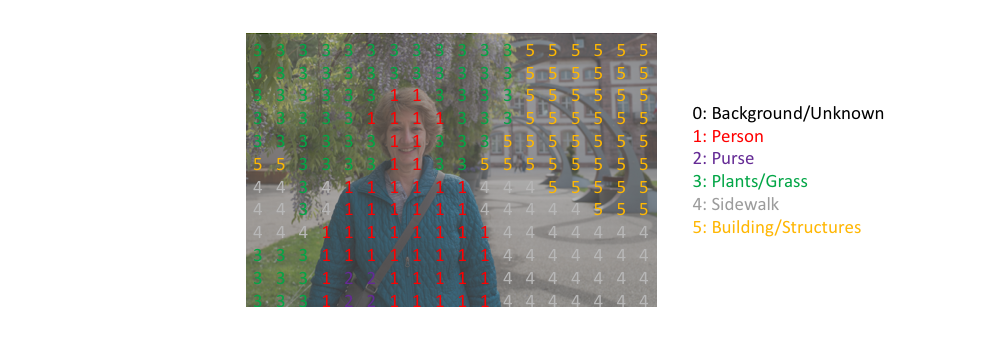
\includegraphics[width=.8\textwidth]{fig/L2/Screen-Shot-2018-05-16-at-9.36.38-PM.png}
\end{figure}
{\tiny \href{https://www.jeremyjordan.me/semantic-segmentation/}{ Images from JEREMY JORDAN}}
\end{frame}

\begin{frame}{Image segmentation: one-hot-encoding}
    Operation of "one-hot encoding" replaces class digits with probability vectors.
    \begin{figure}
   \centering
    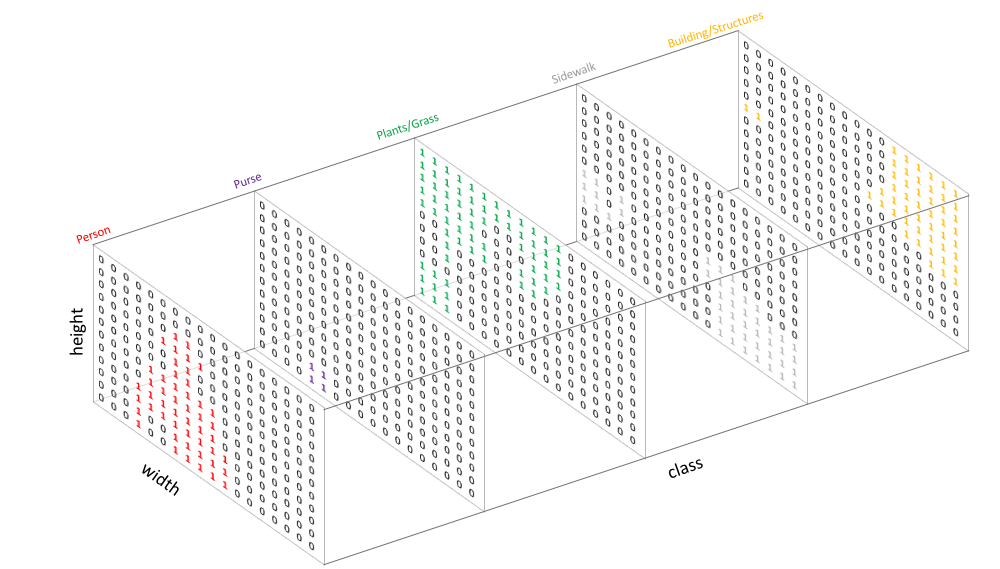
\includegraphics[width=.8\textwidth]{fig/L2/Screen-Shot-2018-05-16-at-9.36.00-PM.png}
\end{figure}
{\tiny \href{https://www.jeremyjordan.me/semantic-segmentation/}{ Images from JEREMY JORDAN}}
\end{frame}

\begin{frame}{Naive CNN for image segmentation}
    Size of convolution filters and padding is selected such that the input image size is preserved (padding='same').
    \begin{figure}
   \centering
    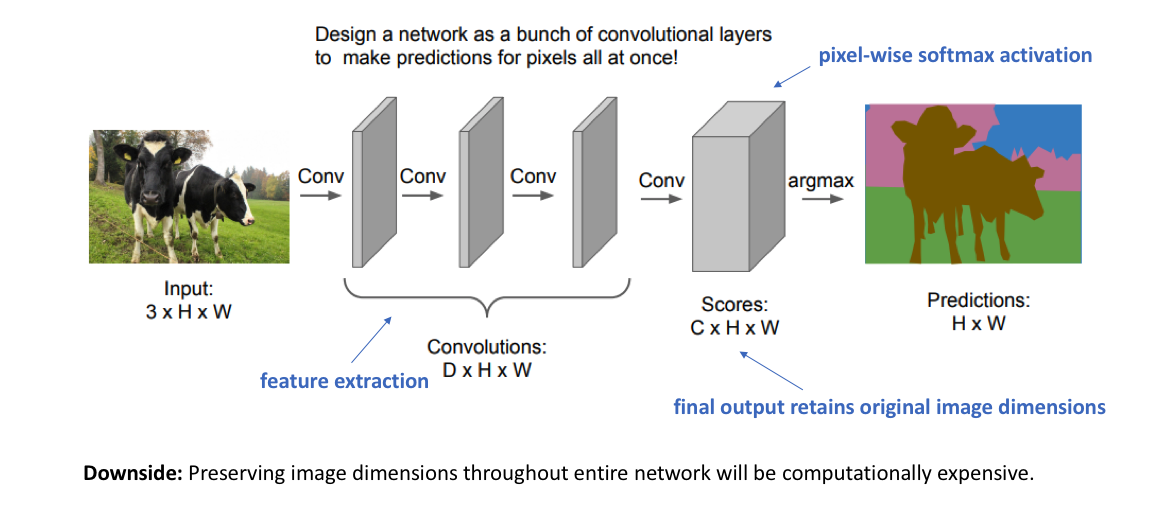
\includegraphics[width=.9\textwidth]{fig/L2/Screen-Shot-2018-05-19-at-12.32.20-PM.png}
\end{figure}
{\tiny \href{https://www.jeremyjordan.me/semantic-segmentation/}{ Images from JEREMY JORDAN}}
\end{frame}

\begin{frame}{Deep CNN for image segmentation}
    Another approach: convolution + DOWN-sampling + convolution + UP-sampling.
    \begin{figure}
   \centering
    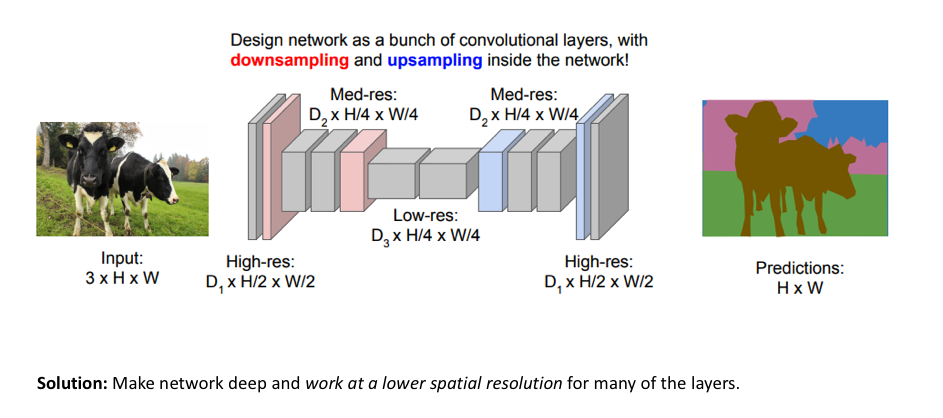
\includegraphics[width=.9\textwidth]{fig/L2/Screen-Shot-2018-05-16-at-10.33.29-PM.png}
\end{figure}
{\tiny \href{https://www.jeremyjordan.me/semantic-segmentation/}{ Images from JEREMY JORDAN}}
\end{frame}

\begin{frame}{Upsampling using "Transpose Convolution"}
Often "Transpose Convolution" is used for upsampling. A convolution filter is applied to small input image with large padding and/or with strides. The example here shows: Padding = 2, Stride = 0.

Blue - input image, gray - filter, green - output image.
    \begin{figure}
        \centering
\multiinclude[<+->][format=png,graphics={width=0.3\textwidth}]{fig/L2/animated/YyCu2}
    \end{figure}
{\tiny \href{https://github.com/vdumoulin/conv_arithmetic}{ Images from fvisin Francesco}}
\end{frame}

\begin{frame}{Upsampling using "Transpose Convolution"}
Padding = 2, Stride = 1.

Blue - input image, gray - filter, green - output image.
    \begin{figure}
        \centering
\multiinclude[<+->][format=png,graphics={width=0.3\textwidth}]{fig/L2/animated/no_padding_strides_transposed}
    \end{figure}
{\tiny \href{https://github.com/vdumoulin/conv_arithmetic}{ Images from fvisin Francesco}}
\end{frame}

\begin{frame}{U-net architecture}
    \alert{U-net} is very well known CNN architecture for semantic segmentation (34K citations).

\begin{thebibliography}{GBC16}

\bibitem[OR2015]{Olaf_Ronneberger_2015}
Olaf Ronneberger, Philipp Fischer and Thomas Brox, \emph{{U-Net: Convolutional Networks for Biomedical Image Segmentation}}, arXiv, 2015.
\end{thebibliography}

    \begin{figure}
        \centering
        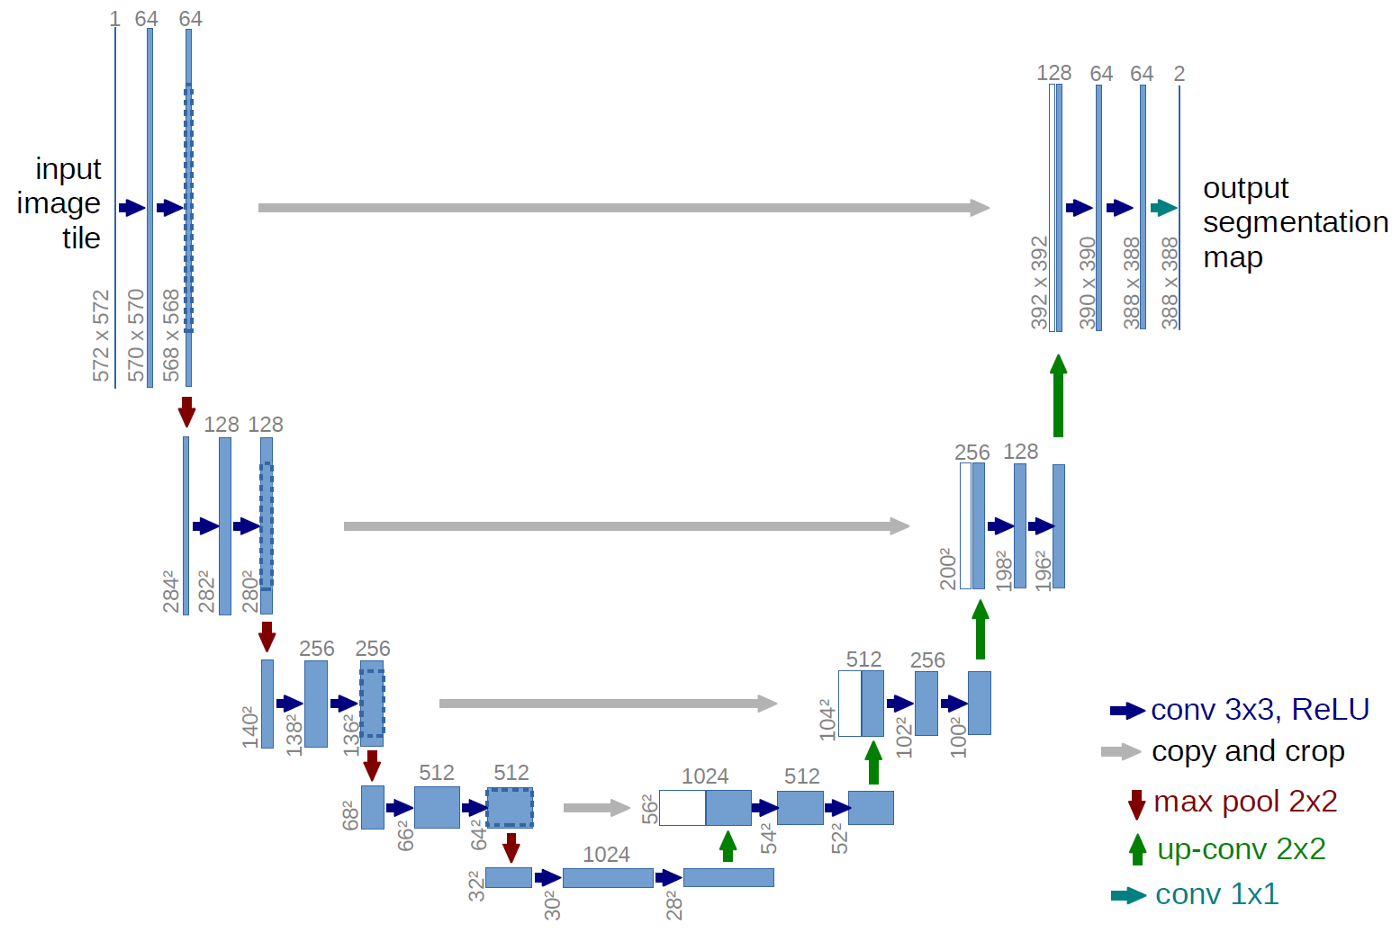
\includegraphics[width=.6\textwidth]{fig/L2/unet.png}
    \end{figure}
\end{frame}

\section{Regularization of neural network training}

\begin{frame}{Under-fitting, Over-fitting}
    From the regression lecture we remember that we can \alert{under-fit} or \alert{over-fit} our model when we have too few or too many parameters.

    \begin{figure}
        \centering
        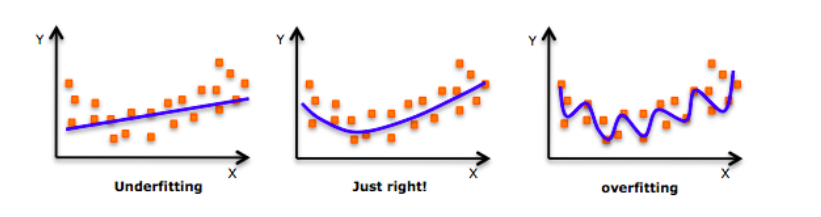
\includegraphics[width=.9\textwidth]{fig/L2/underfitting_overfitting.png}
    \end{figure}
\end{frame}

\begin{frame}{Over-fitting of CNN}
    Training of a network (also CNN) is an iterative process. At each iteration we compute a train and a validation loss. Observing dynamics of train and validation loss can help detect over-fitting.

    \begin{figure}
        \centering
        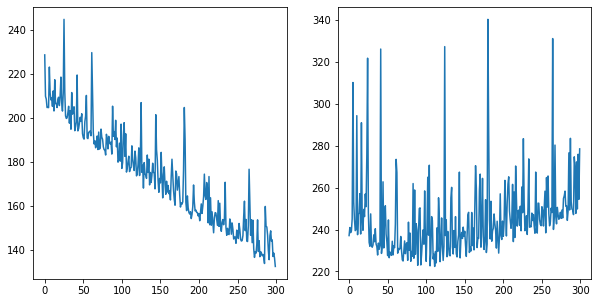
\includegraphics[width=.8\textwidth]{fig/L2/regularization_real.png}
        
        {\tiny The figure shows dynamics of train loss (left) and validation loss (right).}
    \end{figure}
\end{frame}

\begin{frame}{L2-regularization}
    L2-regularization is a term in the loss calculation that penalizes not only error of prediction but also \alert{square} of the model parameters. L2-regularization is used quite often as it reduces too high values of parameters.

    \begin{figure}
        \centering
        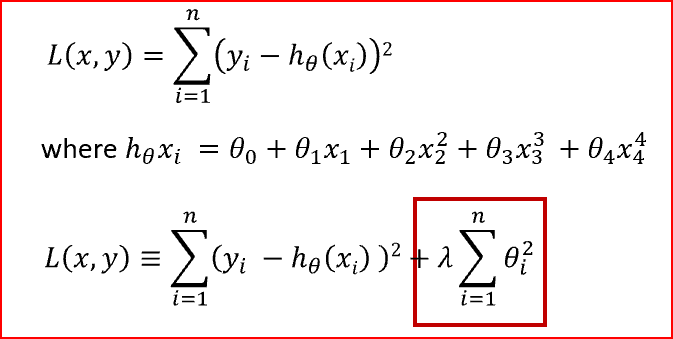
\includegraphics[width=.8\textwidth]{fig/L2/l2_reg.png}
        
    \end{figure}
\end{frame}

\begin{frame}{L1-regularization}
    L1-regularization penalizes \alert{modulus} of the model parameters. L1-regularization is less famous as too many parameters may turn to zero.

    \begin{figure}
        \centering
        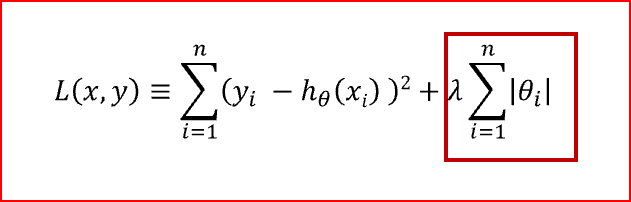
\includegraphics[width=.8\textwidth]{fig/L2/l1_reg.png}
        
    \end{figure}
\end{frame}


\begin{frame}{Too complex network}
    When the network is too complex (too many neurons and connections between them) the classification task can be over-fitted.

    \begin{figure}
        \centering
        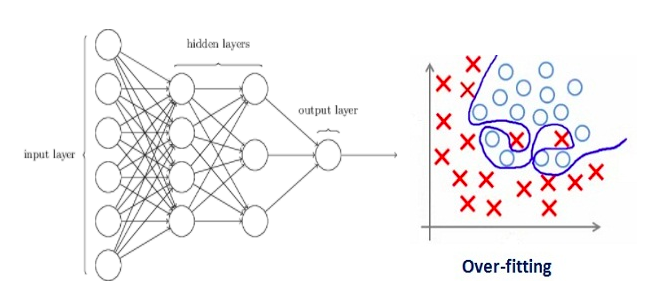
\includegraphics[width=.8\textwidth]{fig/L2/dropout1.png}
        
    \end{figure}
\end{frame}

\begin{frame}{Too simple network}
    When the network is too simple (too few neurons and connections between them) the classification task can be under-fitted.

    \begin{figure}
        \centering
        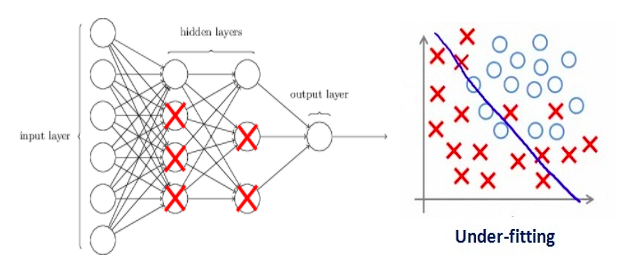
\includegraphics[width=.8\textwidth]{fig/L2/dropout2.png}
        
    \end{figure}
\end{frame}

\begin{frame}{Optimal network?}
    What is the optimal network for finding optimal solution and not over-fitting.

    \begin{figure}
        \centering
        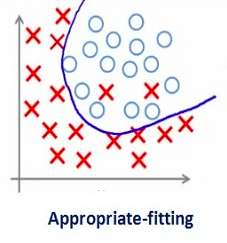
\includegraphics[width=.6\textwidth]{fig/L2/dropout3.png}
        
    \end{figure}
\end{frame}

\begin{frame}{Dropout}
A \alert{Dropout} layer is added to the model. Random neurons are removed from this layer at each epoch of training. The fraction of remove neurons is called \alert{dropout rate}.
    \begin{figure}
        \centering
\multiinclude[<+->][format=png,graphics={width=0.7\textwidth}]{fig/L2/animated/dropout_anim}       
    \end{figure}
\end{frame}

\begin{frame}{Results of model regularization}
    After the regularization options are added the train loss is higher, but the model is not overfitted.

    \begin{figure}
        \centering
        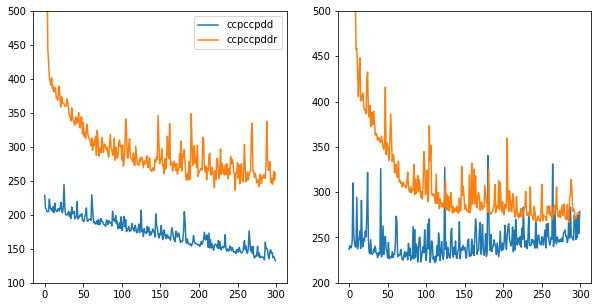
\includegraphics[width=.6\textwidth]{fig/L2/regularization_real2.png}
        
    \end{figure}
\end{frame}

\section{Data for the practical exercise}

\begin{frame}{Data sources and task}
    Data sources:
    \begin{itemize}
        \item Sentinel-1 SAR. 1 pixel: 40m. Two polarisations: HH and HV.
        \item Sea ice concentration. 1 pixel: 12 km. Range of SIC: 0 - 100
    \end{itemize}
    \begin{figure}
        \centering
        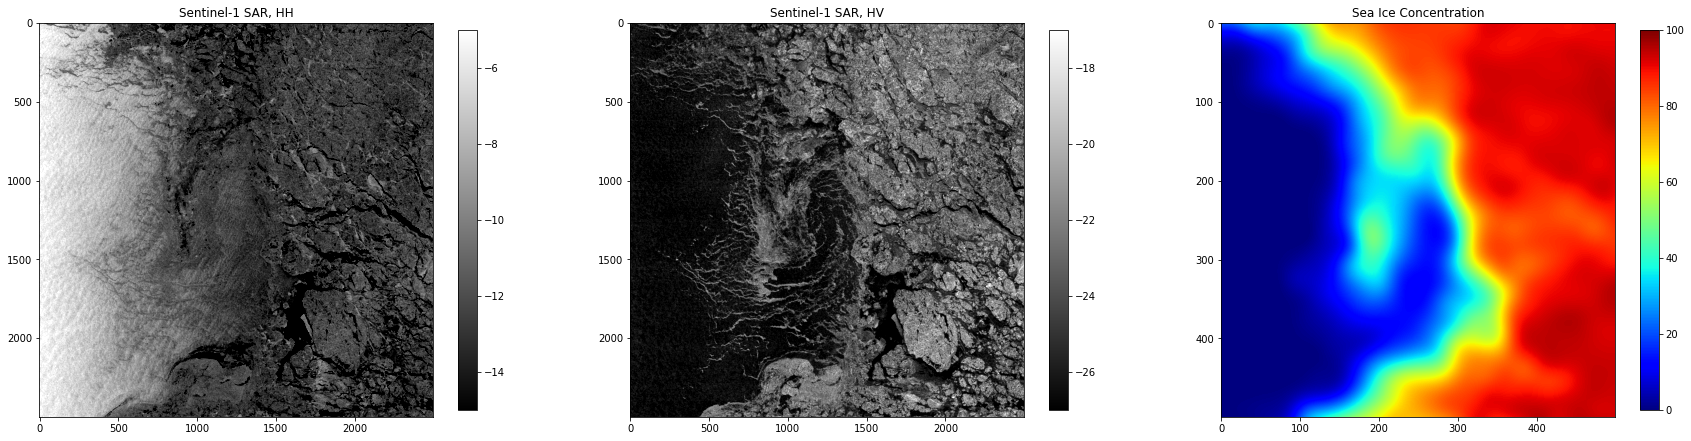
\includegraphics[width=.99\textwidth]{fig/L2/input_data_p5.png}
    \end{figure}
\end{frame}

\begin{frame}{Collocated HV and SIC}
    \begin{figure}
        \centering
        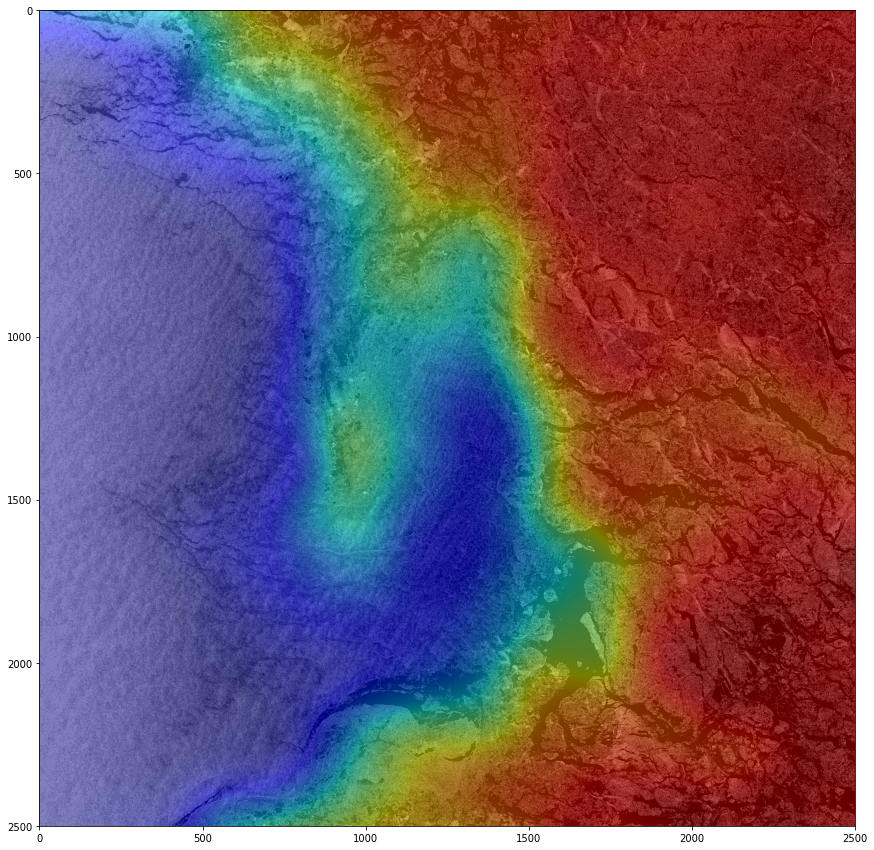
\includegraphics[width=.8\textwidth]{fig/L2/inp_data_p5_colocated.png}
    \end{figure}
\end{frame}

\end{document}
%%%%%%%%%%%%%%%%%%%%%%%%%%%%%%%%%%%%%%%%%%



